% {{{ Packages

% {{{ Versions
% version écran
\documentclass{beamer}

% version présentation
%\documentclass[8pt]{beamer}
%\usepackage{pgfpages}
%\setbeamertemplate{note page}[plain]
%\setbeameroption{show notes on second screen=left}

% version orateur
%\documentclass[9pt]{beamer}
%\usepackage{pgfpages}
%\pgfpagesuselayout{2 on 1}[a4paper,border shrink=5mm]
%\setbeameroption{show only notes}

% version spectateur
%\documentclass[handout]{beamer}
%\usepackage{handoutWithNotes}
%\pgfpagesuselayout{1 on 1 with notes}[a4paper,border shrink=5mm]
% }}}

\usepackage[utf8]{inputenc}
\usepackage[french]{babel}
\usepackage{tikz}
\usepackage{caption}
\usetheme{Goettingen}

% }}}
% {{{ Commands
\makeatletter
\def\ft@overlay{}

\addtobeamertemplate{footline}{}
{
    \lineskiplimit0pt
    \begin{tikzpicture}[remember picture,overlay]
        \ft@overlay
    \end{tikzpicture}
    \gdef\ft@overlay{}
}

\newcommand<>{\addtooverlay}[1]{
    \only#2{
      \expandafter\gdef\expandafter\ft@overlay\expandafter{\ft@overlay
          \draw[fill=black,opacity=0.70]
              (current page.north east) rectangle (current page.south west);
          \node[text=white,font=\Huge] at (current page.center) {
              #1
          };
      }
    }
    \pause
}
% }}}

\title{Tester son API REST}
\author{Sanpi}
\date{21 avril 2016}

\begin{document}
% {{{ Titre
\begin{frame}
    \titlepage
\end{frame}
% }}}

% {{{ PHPUnit
\begin{frame}
    \frametitle{Précédemment}
\end{frame}

\note[itemize] {
    \item Lors du dernier SfPot, suite à la présentation très intéressante sur
        l’architecture REST, la question de comment tester automatiquement une
        telle application a été posée.
    \item La première réponse qui a été donnée, sans grande surprise, est
        d’utiliser phpunit ; et de tester la réponse JSON avec des assertEquals
}

\begin{frame}
    \frametitle{Précédemment}

    \begin{itemize}[<+->]
        \item PHPUnit
    \end{itemize}

    \addtooverlay<.(1)>{
        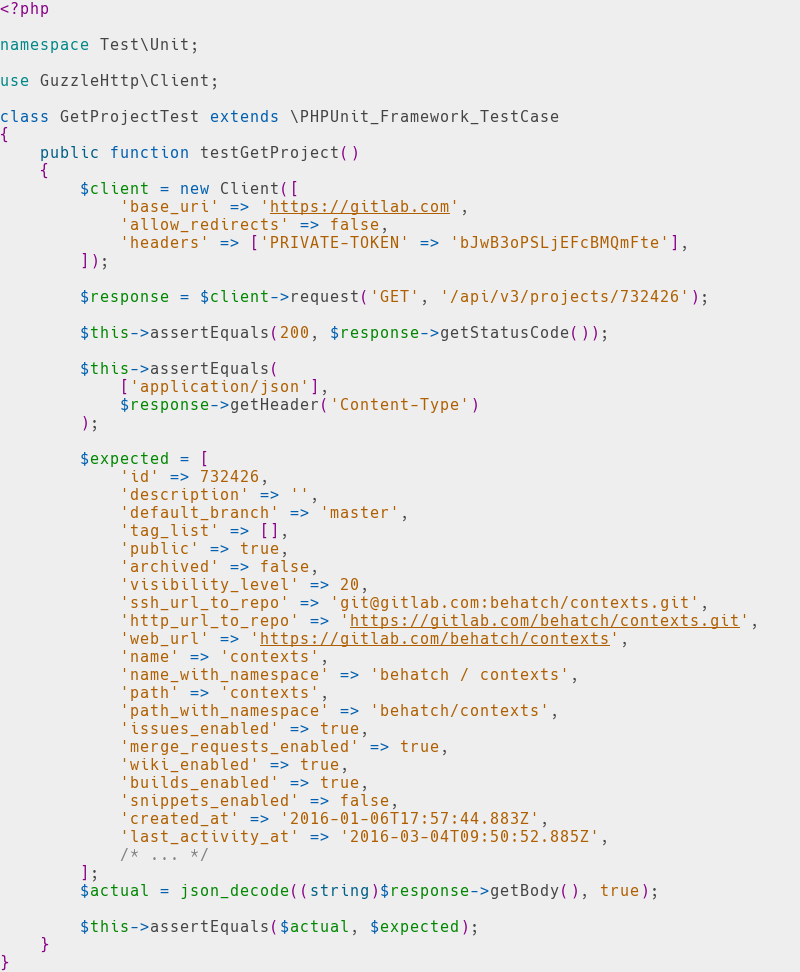
\includegraphics[scale=0.28]{images/phpunit-get}
    }
\end{frame}

\note[itemize] {
    \item Alors pour vous donner une idée, voici à quoi ça ressemble. Ici il
        s’agit de récupérer les informations d’un projet sous gitlab.
    \item Je ne sais pas ce que vous en pensez, mais je trouve ça difficile à
        comprendre.
    \item Alors qu’on soit bien d’accord, il s’agit de tests automatisés, c’est
        donc une bonne chose. Cela prouve que vous êtes capable de déployer
        votre projet automatiquement et on évite les régressions.
    \item Mais ça me semble compliqué à maintenir, et il est fort probable que
        vos tests deviennent inutiles avec le temps, car non maintenus.
    \item Donc vous l’aurez compris, ce n’est pas la solution dont je suis venu
        vous présenter ce soir.
}
% }}}

% {{{ Behat
\begin{frame}
    \frametitle{Behat}
\end{frame}

\note[itemize] {
    \item Je vais plutôt vous parler de behat.
    \item Qui utilise behat ?
}

\begin{frame}
    \frametitle{Behat}

    \begin{itemize}
        \item \em{\alert<3>{Behavior Driven Development} \alert<4>{framework}
            for \alert<2>{PHP}}

        %\addtooverlay<.(5)>{
        %    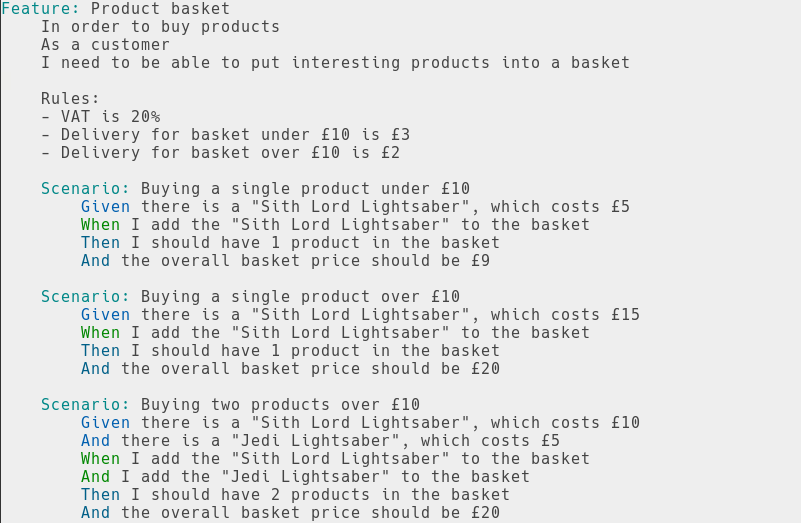
\includegraphics[scale=0.28]{images/behat}
        %}
    \end{itemize}
\end{frame}

\note[itemize] {
    \item D’après le site officiel, behat est un framework pour le développement
        piloté par le comportement pour PHP.
    \item Donc, reprenons. PHP, ça va pour tout le monde.
    \item Behavior Driven Development, ou BDD. C’est une méthode de
        développement agile. Pour résumé en deux phrases, il s’agit d’encourager
        la communication entre les développeurs et les intervenants non
        techniques (ce qui implique l’utilisation d’un langage proche du langage
        naturel) ; et deuxièmement de se focaliser sur le comportement de vos
        utilisateurs.
    \item Et enfin framework, parce que behat n’est qu’un cadre de développement
        qui de base ne sait rien faire.
    \item Enfin rien, c’est réducteur, il est capable d’exécuter des scénarios
        de tests mais il ne possède pas d’action.
}
% {{{ Étendre behat
\begin{frame}
    \frametitle{Étendre behat}
\end{frame}

\begin{frame}
    \frametitle{Étendre behat}

    \begin{itemize}[<+->]
        \item MinkExtension
        \item Symfony2Extension
        \item …
        \item Behatch
        \begin{itemize}
            \item<5-> \alert<5>{Browser}
            \addtooverlay<.(2)>{
                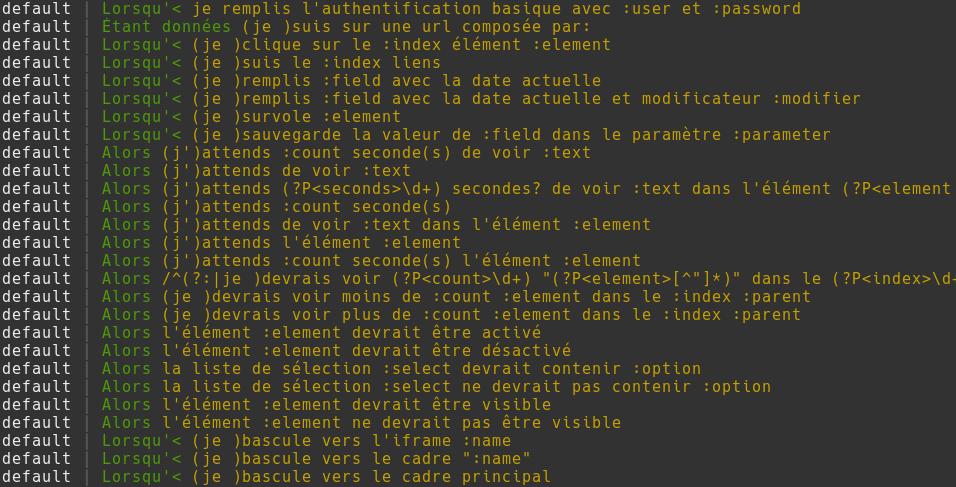
\includegraphics[scale=0.28]{images/behatch-browser-mini}
            }
            \item<7-> \alert<7>{Table}
            \addtooverlay<.(3)>{
                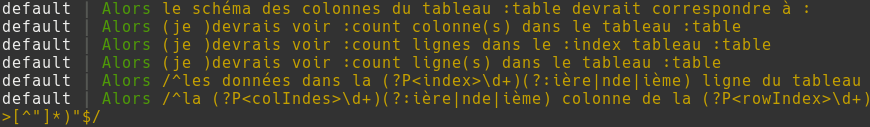
\includegraphics[scale=0.28]{images/behatch-table-mini}
            }
            \item<9-> \alert<9>{Debug}
            \addtooverlay<.(4)>{
                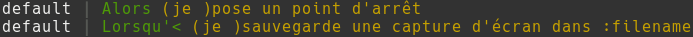
\includegraphics[scale=0.28]{images/behatch-debug}
            }
            \item<11-> \alert<11>{System}
            \addtooverlay<.(5)>{
                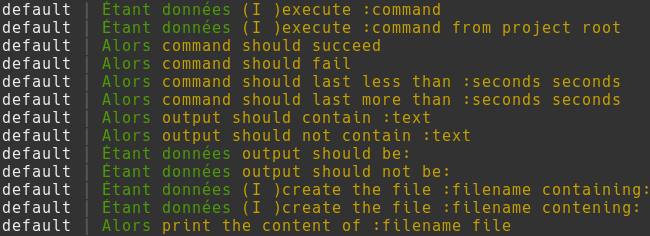
\includegraphics[scale=0.28]{images/behatch-system}
            }
            \item<13-> \alert<13>{Xml}
            \addtooverlay<.(6)>{
                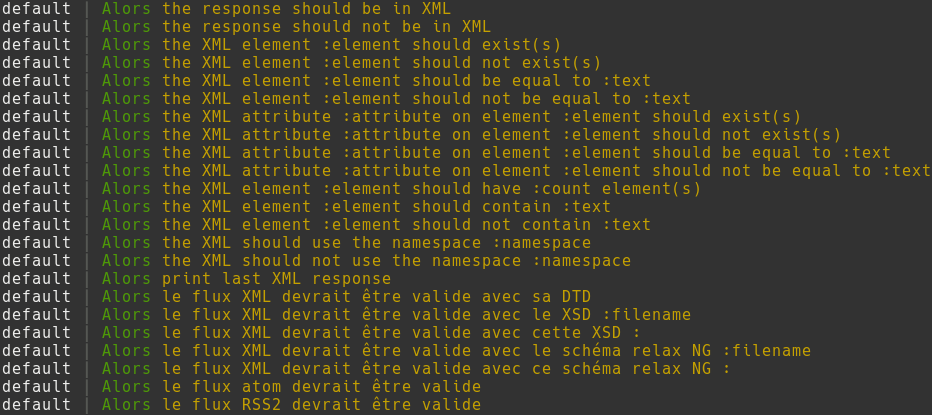
\includegraphics[scale=0.28]{images/behatch-xml}
            }
            \item<15-> \alert<15>{REST}
            \item<15-> \alert<15>{Json}
        \end{itemize}
    \end{itemize}
\end{frame}

\note[itemize] {
    \item Bien évidement il est possible de développer des extensions que vont
        apporter des actions.
    \item Par exemple Mink qui permet de faire des tests dans un navigateur ;
    \item Ou encore une extension pour symfony qui permet de manipuler
        simplement vos services dans vos actions ;
    \item Il en existe bien sûr d’autres, mais je vais vous parler de celle que
        je maintient depuis 4 ans maintenant ;
    \item Il s’agit de behatch, qui regroupe des divers actions, c’est un
        fourre-tout composer de différentes catégories.
    \item Browser ajoute des actions en plus pour mink, comme répondre à une
        authentification basique ou encore naviguer dans les iframes d’une page.
    \item Table se focalise sur les tableaux html ;
    \item Debug, extrêmement pratique permet de faire une pause dans les tests
        (si vous lancez vos tests dans firefox, le navigateur reste ouvert, et
        vous pouvez inspecter la page). Cette extension permet de prendre
        automatiquement une capture d’écran lorsqu’un scénario nécessitant
        du javascript échoue.
    \item System permet de lancer des commandes ou encore créer un fichier
    \item XML pour tester vos sorties au format XML, valider à l’aide d’une DTD.
    \item et enfin, les deux derniers REST et Json, qui vont tout
        particulièrement nous intéressés aujourd’hui.
}
%}}}

% {{{ Rest
\begin{frame}
    \frametitle{REST}
\end{frame}

\begin{frame}
    \frametitle{REST}

    \addtooverlay<.(1)>{
        
\includegraphics[scale=0.28]{images/behat-rest-1}
    }
    \addtooverlay<.(1)>{
        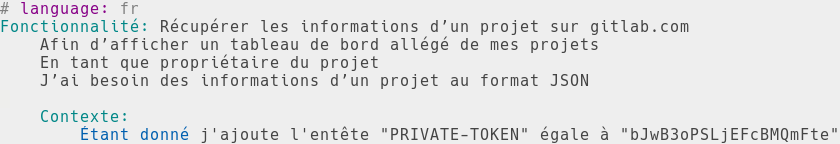
\includegraphics[scale=0.28]{images/behat-rest-2}
    }
    \addtooverlay<.(1)>{
        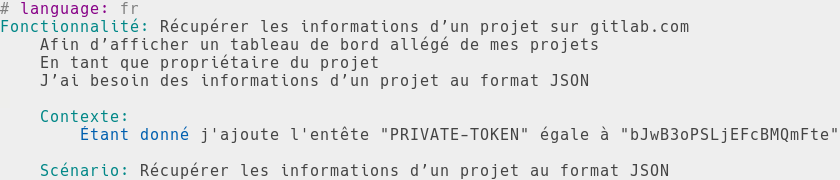
\includegraphics[scale=0.28]{images/behat-rest-3}
    }
    \addtooverlay<.(1)>{
        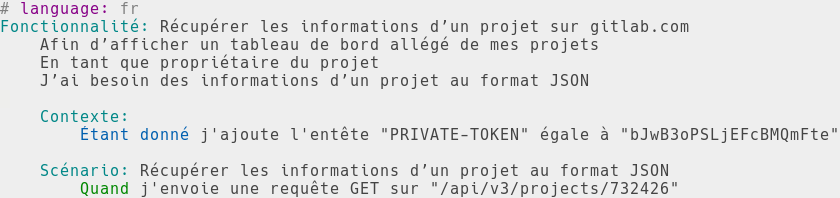
\includegraphics[scale=0.28]{images/behat-rest-4}
    }
    \addtooverlay<.(1)>{
        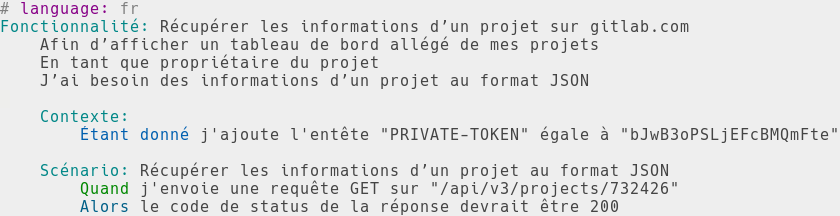
\includegraphics[scale=0.28]{images/behat-rest-5}
    }
    \addtooverlay<.(1)>{
        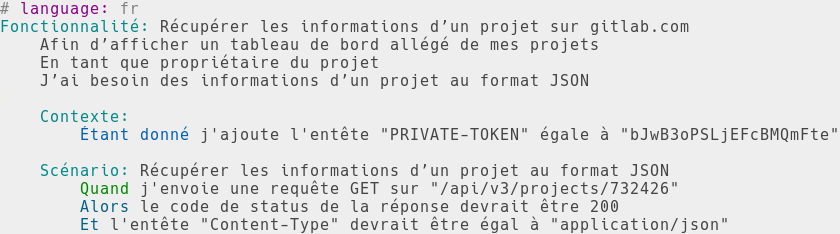
\includegraphics[scale=0.28]{images/behat-rest-6}
    }
\end{frame}

\note[itemize] {
    \item Que je vais vous présenter en reprenant l’exemple du début sous phpunit
    \item On commence notre fichier de test en précisantque nous allons
        utiliser la langue française
    \item Et nous décrivons notre fonctionnalité : ce que l’on souhaite faire,
        pourquoi, et de quel point de vue.
    \item Ensuite, le contexte permet d’exécuter une action avant chaque
        scénario. c’est l’équivalent du setUp() dans les tests unitaires. Ici on
        configure l’entête HTTP PRIVATE-TOKEN afin de nous authentifier.
    \item On crée un nouveau scénario, et on décrit ce que l’on va tester
    \item Et c’est parti, on commence par envoyer une requête GET
    \item On vérifie que son code de status est bien 200
    \item Et que l’entête "Content-Type" correspond à du JSON
    \item Voilà pour la partie REST. Il y a quelques actions supplémentaires
        mais on vient de voir l’esentiel.
}
%}

% {{{ JSON
\begin{frame}
    \frametitle{JSON}
\end{frame}

\note[itemize] {
    \item Passons à la partie JSON
}

\begin{frame}
    \frametitle{JSON}

    \addtooverlay<.(1)>{
        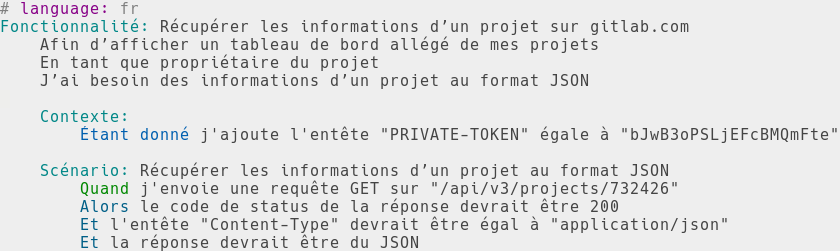
\includegraphics[scale=0.28]{images/behat-json-1}
    }
    \addtooverlay<.(1)>{
        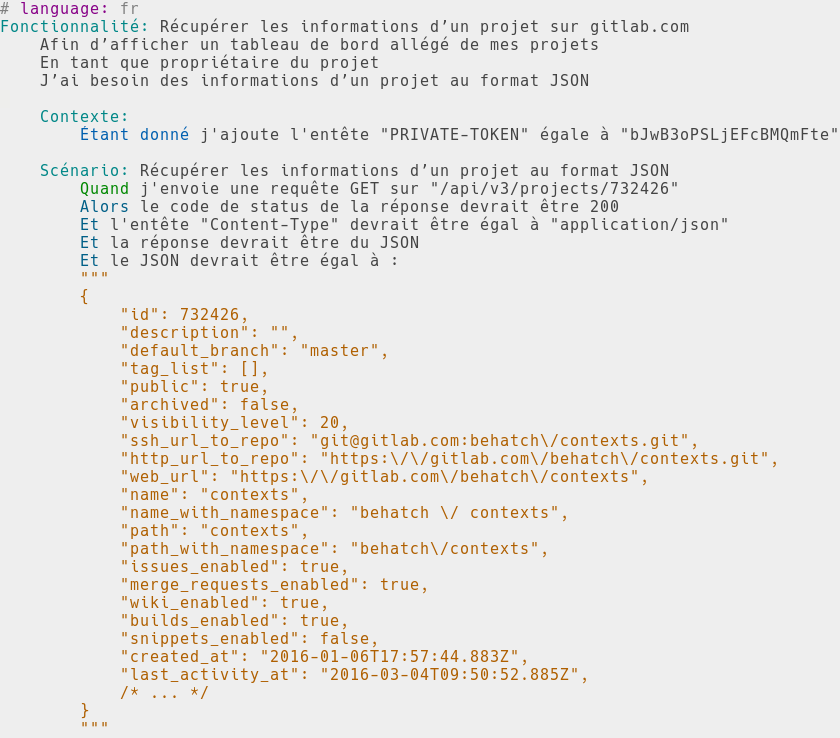
\includegraphics[scale=0.28]{images/behat-json-2}
    }
\end{frame}

\note[itemize] {
    \item On s’assure que la réponse est bien du JSON, sans erreur de syntaxe
    \item Et enfin, on vérifie le contenu du JSON
    \item Voilà, nous avons le même test qu’avec phpunit mais écrit avec behat.
        C’est tout de même plus lisible et en plus c’est documenté
    \item Mais si vous avez la bonne idée de générer vos jeux de tests
        automatiquement, avec des outils tel que faker, tester un JSON à
        l’identique, ce n’est pas possible puisqu’à chaque fois que vous allez
        exécuter un test, les données vont changer.
    \item La solution pourait être d’utiliser des expressions rationnelles, mais
        mélanger à du JSON ça risque de devenir rapidement illisible.
    \item Donc on va s’inspirer d’une très bonne idée mise en place pour le
        format XML : les schémas de validation.
}
% {{{ Schéma
\begin{frame}
    \frametitle{Schéma JSON}
\end{frame}

\begin{frame}
    \frametitle{Schéma JSON}

    \begin{itemize}[<+->]
        \item \url{http://json-schema.org}

        \addtooverlay<.(1)>{
            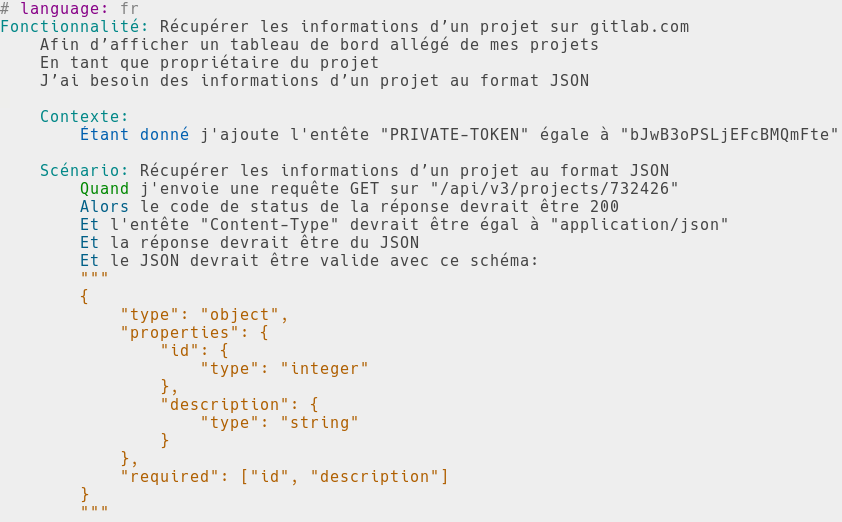
\includegraphics[scale=0.28]{images/behat-schema}
        }
        \addtooverlay<.(1)>{
            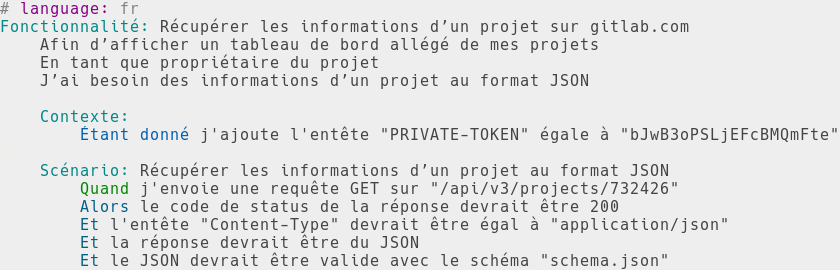
\includegraphics[scale=0.28]{images/behat-schema-file}
        }
        \addtooverlay<.(1)>{
            
\includegraphics[scale=0.28]{images/schema}
        }

        \item \url{http://jsonschema.net}
    \end{itemize}
\end{frame}

\note[itemize] {
    \item Cela exiset également pour JSON, c’est documenté sous forme de RFC (encore
        à l’état de brouillon). Vous trouvez toutes les info sur ce site.
    \item L’utilisation se passe de commentaire.
    \item Concernant le schéma, on précise simplement le noms des propriétés,
        leurs type et s’ils sont obligatoire.
    \item Par contre les schema peuvent rapidement l’alongé, je vous conseille de
        mettre le schéma dans un fichier séparé.
    \item Comme ça on récupère la coloration syntaxique.
    \item En plus, une fois qu’on a nos schéma, on peux les réutiliser. Par
        exemple pour valider les réponse pour un outils en ligne de commande.
    \item Et comme ça peux être fastidieu d’écrire des schémas à la main, il
        existe ce site pour vous aider.
}
% }}}
% {{{ Résumé
\begin{frame}
    \frametitle{Résumé}
\end{frame}

\begin{frame}
    \frametitle{Résumé}

    \addtooverlay<.(1)>{
        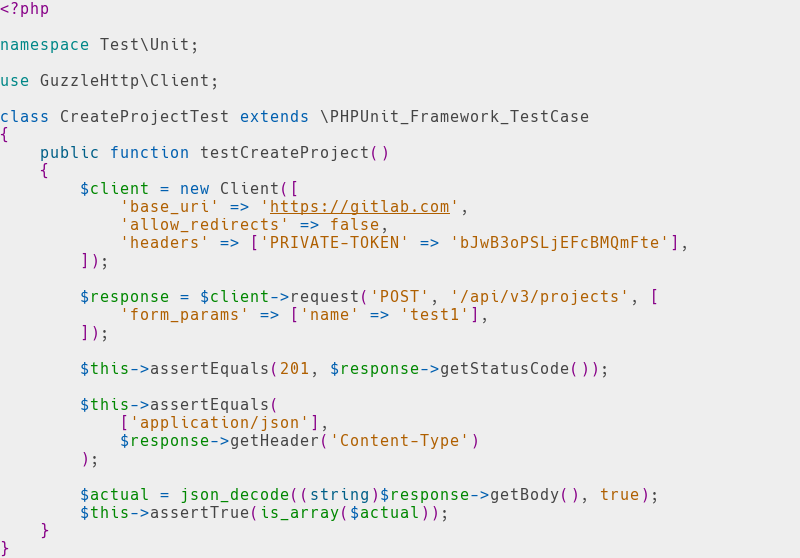
\includegraphics[scale=0.28]{images/phpunit-post}
    }
    \addtooverlay<.(1)>{
        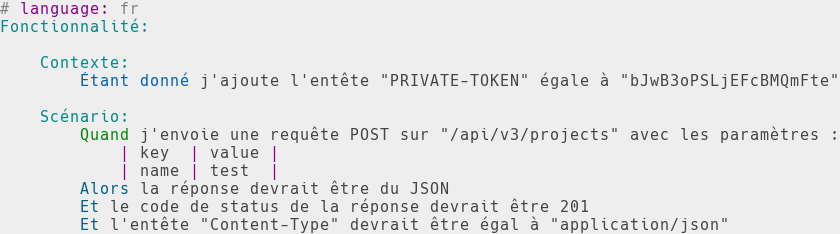
\includegraphics[scale=0.28]{images/behat-post}
    }
\end{frame}

\note[itemize] {
    \item En guise de résumé, je vous propose Un autre exemple, avec la création
        d’un nouveau projet sous gitlab
    \item Voici la version phpunit. Donc une requête POST avec le paramètre
        name. On vérifie le code de status de la réponse et l’entête
        Content-Type.
    \item Et voici la même chose avec behat.
}
%}}}
% {{{ Tester behatch
\begin{frame}
    \frametitle{Tester behatch}
\end{frame}

\note[itemize] {
    \item Comme j’espère vous avoir convaincu, voici quelques solutions pour
        tester rapidement behatch.
}

\begin{frame}
    \frametitle{Tester behatch}

    \begin{itemize}
        \item composer -sdev create-project …
        \begin{itemize}
            \item<1-> \alert<1>{behatch/skeleton}
            \item<2-> \alert<2>{sanpi/spore}
            \item<2-> \alert<2>{sanpi/symbiose}
        \end{itemize}
    \end{itemize}
\end{frame}

\note[itemize] {
    \item Dans le projet behatch vous avez  un squelette minimaliste, avec la
        configuration, le composer.json et les dossiers vides.
    \item Si vous voulez allez plus loin, j’ai également deux autres modèles, le
        premier pour silex, le second pour symfony3 qui inclue behatch.
        Ils sont basé sur mes préférences, mais au moins il peuvent vous aider à
        mettre en place behat.
}
%}}}

% {{{ Défauts
\begin{frame}
    \frametitle{Défauts}
\end{frame}

\note[itemize] {
    \item Pour être totalement honête avec vous, il y a quand même quelques
        soucis à utiliser behat pour tester une API REST.
}

\begin{frame}
    \frametitle{Défauts}

    \begin{itemize}[<+->]
        \item Détournement de behat
        \addtooverlay<.(1)>{
            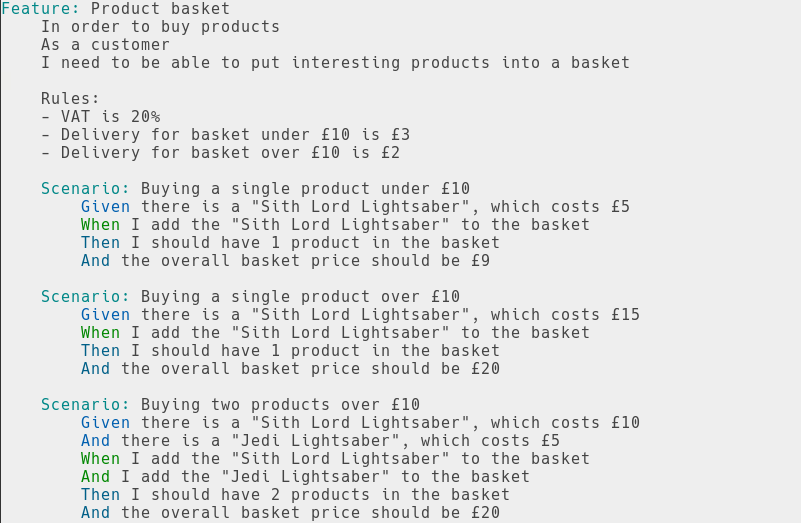
\includegraphics[scale=0.28]{images/behat}
        }
        \item Client http problèmatique
    \end{itemize}
\end{frame}

\note[itemize] {
    \item Premièrement, on détournement behat de sa fonction première.  Du point
        de vu du BDD, on est trop technique. On peux augmenter l’abstration des
        test.
    \item Pour vous donner une idée, voici à quoi ressemble un test avec behat,
        issue de la documentation. Le niveau d’abstraction est bien supérieur.
    \item Oui, mais ça marche tellement bien, que je ne vois pas pourquoi s’en
        privé.
    \item Et si on y réfléchi, le client de notre API, ce n’est pas le client
        final, généralement c’est un autre développeur qui en a besoin pour
        alimenter en donnée le front office. Donc on parle bien le même langage.
    \item Deuxième soucis, au niveau des actions REST, le client http
        pose problème. On utilise mink qui n’est pas fait pour ça.
}
% }}}

% {{{ Questions
\begin{frame}
    \frametitle{Questions}

    \begin{figure}
        
\includegraphics{images/qrcode}
        \captionsetup{labelformat=empty}
        \caption{
            \scriptsize{https://github.com/sanpii/slides/releases/download/sfpot/behat-rest.pdf}
        }
    \end{figure}
\end{frame}
% }}}
\end{document}
